\documentclass[11pt]{article}
\usepackage{amsmath, amssymb, amsthm, amsfonts,cite,alltt}
\usepackage[english]{babel}
\usepackage{graphicx}
\usepackage{caption}
\usepackage[list=true,listformat=simple]{subcaption}
\renewcommand{\tt}{\texttt}

\newtheorem{theorem}{Theorem}[section]
\newtheorem{lemma}[theorem]{Lemma}
\newtheorem{proposition}[theorem]{Proposition}
\newtheorem{corollary}[theorem]{Corollary}


\newenvironment{definition}[1][Definition]{\begin{trivlist}
\item[\hskip \labelsep {\bfseries #1}]}{\end{trivlist}}
\newenvironment{example}[1][Example]{\begin{trivlist}
\item[\hskip \labelsep {\bfseries #1}]}{\end{trivlist}}
\newenvironment{remark}[1][Remark]{\begin{trivlist}
\item[\hskip \labelsep {\bfseries #1}]}{\end{trivlist}}

% Complex \xxx for making notes of things to do.  Use \xxx{...} for general
% notes, and \xxx[who]{...} if you want to blame someone in particular.
% Puts text in brackets and in bold font, and normally adds a marginpar
% with the text ``xxx'' so that it is easy to find.  On the other hand, if
% the comment is in a minipage, figure, or caption, the xxx goes in the text,
% because marginpars are not possible in these situations.
{\makeatletter
 \gdef\xxxmark{%
   \expandafter\ifx\csname @mpargs\endcsname\relax % in minipage?
     \expandafter\ifx\csname @captype\endcsname\relax % in figure/caption?
       \marginpar{xxx}% not in a caption or minipage, can use marginpar
     \else
       xxx % notice trailing space
     \fi
   \else
     xxx % notice trailing space
   \fi}
 \gdef\xxx{\@ifnextchar[\xxx@lab\xxx@nolab}
 \long\gdef\xxx@lab[#1]#2{\textbf{[\xxxmark #2 ---{\sc #1}]}}
 \long\gdef\xxx@nolab#1{\textbf{[\xxxmark #1]}}
 % This turns them off:
 % \long\gdef\xxx@lab[#1]#2{}\long\gdef\xxx@nolab#1{}%
}



\setlength{\parindent}{0.0in}
\setlength{\parskip}{0.1in}
\usepackage[margin=1in]{geometry}
\begin{document}

\title{The Computational Complexity of Push-Pull Block Puzzles}
%\author{Erik Demaine\thanks{MIT Computer Science and Artificial Intelligence Laboratory, 32 Vas-
%sar Street, Cambridge, MA 02139, USA} \and Isaac Grosof\footnotemark[1]  \and Jayson Lynch\footnotemark[1]}
%\date{\today}
%\maketitle

%%Upgrade Trees might be hard, also some sort of inventory thing might be interested. Then we should hit Cookie Clicker and other simulation games (Sim City).

\begin{abstract}
This paper proves that push-pull block puzzles in 3D are PSpace-Complete to solve and push-pull block puzzles in 2D with thin walls are NP-Hard to solve. Push-pull block puzzles are a game, and motion planning problem, similar to Sokoban, that involves moving a `robot' on a grid with obstacles. The obstacles cannot be traversed by the robot, but some can be pushed or pulled by the robot into adjacent squares. Thin walls prevent movement between two adjacent squares. This work follows in a long line of algorithms and complexity work on similar problems \cite{PushPull91}\cite{Push100}\cite{Push*00}\cite{PushPushk04}\cite{non-crossing01}\cite{DO92}\cite{Push2F02}\cite{Sokoban98}\cite{DZ96}\cite{Pull10}. The 2D push-pull block puzzle shows up in a number of video games, including The Legend of Zelda, thus implying a number of other results. This variant of block pushing puzzles is of particular interest to the authors because it is fully reversible, meaning the inverse of any action that has been taken is valid.
\end{abstract}

\section{Introduction} 

This work builds on a long line of work on the mathematics of games and puzzles, primarily, the recent work in the computational complexity of video games.  We also give a new result showing that block pushing puzzles, like Sokaban, which also include the ability to pull blocks are NP-Hard. This result also proves a number of other games, which have embedded push-pull block puzzles, are NP-Hard.

Games have and continue to be a source of interesting problems for mathematics and computer science. Game playing continues to be a benchmark in the field of AI. The study of economic games has become a large field with applications in online auctions\cite{auctions}, network analysis\cite{Internet}, and voting\cite{colman2013game}. Combinatorial games have lead to algebraic insights such as Conway's Surreal Numbers\cite{Surreal01} and the Sprague-Grundy Theorem\cite{Sprague35}\cite{Grundy39}. More recently, games have been studied from an algorithmic perspective and can be seen as models of computation in examples like Constraint Logic \cite{GPCBook09} and Conway's Game of Life\cite{LifeTuring01}. For a survey of algorithmic combinatorial game theory see Demaine and Hearn's paper\cite{AlgGameTheory_GONC3}. Understanding the computational and algorithmic aspects of games may lead to better understanding of algorithms and problems that share similar properties. For example, certain asymmetries or algebraic properties may be more intuitively obvious in games, such as the relationship between two-player games and quantified boolean formulas\cite{}. In this vein, we are particularly interested in the push-pull block model because it is fully reversible, meaning any sequence of moves in the puzzle can be undone. Reversibility is fundamentally linked to quantum computation and the thermodynamics of computation; thus understanding the difference between reversible and irreversible computation is very relevant. 

Finally, many games and puzzles can also be seen as simplified models of problems in the real world. Thus, solving these problems gives us partial understanding and tools to attack more difficult questions. For example, push-pull block puzzles can be seen as a simplified model of robotic forklifts operating in a warehouse. Complexity results in these very simplified models help us understand what aspects of problems makes them hard and allows us to start differentiating between the complexity that arises from the combinatorics vs the geometry of path planning problems. Similarly, path-planning in dynamic graphs is a complicated problem which occurs every day from traffic to packet routing.




\subsection{Sliding Blocks Related Work}

A significant amount of research has gone into characterizing the complexity of sliding block puzzles. This includes PSpace-Completeness for well known puzzles like Sokaban \cite{Sokoban98} and Rush Hour \cite{RushHour02}. We are specifically interested in block pushing puzzles, which involve a 'robot' that is able to move on a grid and is able to move blocks adjacent to it, typically by 'pushing' or 'pulling' the block. Further, we only address the path planning problem, in which the robot wants to get from a given location $A$ to a target location $B$, rather than the storage problem in which the movable blocks must reach some final configuration. Figure~\ref{BlocksTable} gives a summary of results on block pushing puzzles. 

The problem of motion planning in an environment where blocks may be pushed and pulled is modeled in a very general form in Gordon Wilfong's Motion Planning in the Presence of Movable Obstacles, where he shows a polynomial time algorithm for motion planning with one movable object, NP-Hardness for the general planning problem, and PSpace-Hardness for the storage problem. \cite{PushPull91} His problem, however, deals with continuous motion and polygonal walls and blocks; making the model significantly different from the 1x1 blocks on a grid that is considered for most block pushing puzzles. Marcus Ritt paper \cite{Pull10} addresses the model in which blocks can only be pulled. We primarily build off of Dor and Zwick's work which generalizes Sokoban to include block pulling. They show the block storage problem which includes 2x1 blocks which can be pushed or pulled is PSpace-Complete, and the unit-size block storage where the robot can push at five or more blocks at a time and pull one is NP-Hard\cite{DZ96}. We introduce \emph{thin walls}, which prevent motion between two adjacent empty squares. We prove that all path planning problems in 2D with thin walls, in which the robot can push $k$ blocks and pull $l$ blocks for all $k,l \in \mathbb{Z}^+$ are NP-Hard. As with many of these problems, closing the gap between NP and PSpace remains open. In addition, we prove that all path planning problems in 3D in which the robot can push $k$ blocks and pull $l$ plocks for all $k,l \in \mathbb{Z}^+$ is PSPACE-Complete.

\xxx{check against Erik's notes for completeness}

\begin{table}[ht]
\centering
\begin{tabular}{|l|l|l|l|l|l|l|l|l|}
\hline
\emph{Name} & \emph{Push} & \emph{Pull} & \emph{Block Size} & \emph{Fixed?} & \emph{Path?} & \emph{Sliding} & \emph{Complexity} \\ \hline
\hline
Push-k & k & 0 & Unit & No & Path & min & NP-Hard\cite{Push100} \\ \hline
Push-* & * & 0 & Unit & No & Path  & min & NP-Hard\cite{Push*00} \\ \hline
PushPush-k & k & 0 & Unit & No & Path  & Max & PSpace-Comp.\cite{PushPushk04} \\ \hline
PushPush-* & * & 0 & Unit & No & Path  & Max & NP-Hard\cite{Push*00} \\ \hline
PushPushPush-k & k & 0 & Unit & No & Path  & Max & PSpace-Comp.\cite{} \\ \hline
PushPushPush-* & * & 0 & Unit & No & Path  & Max & NP-Hard\cite{} \\ \hline
Push-kX & k & 0 & Unit & No & No-Cross  & min & NP-Comp.\cite{non-crossing01} \\ \hline
Push-*X & * & 0 & Unit & No & No-Cross  & min & NP-Comp.\cite{non-crossing01} \\ \hline
Push-1F & 1 & 0 & Unit & Yes & Path  & min &  NP-Hard \cite{DO92} \\ \hline
Push-kF & k$\geq 2$ & 0 & Unit & Yes & Path  & min & PSpace-Comp.\cite{Push2F02} \\ \hline
Push-*F & * & 0 & Unit & Yes & Path  & min & PSpace-Comp.\cite{Push2F02} \\ \hline
Sokoban & 1 & 0 & Unit & Yes & Storage  & min & PSpace-Comp.\cite{Sokoban98} \\ \hline
Sokoban$^+$ & k$\geq 2$ & 1 & 2x1 & Yes & Storage  & min & PSpace-Comp.\cite{DZ96} \\ \hline
 & k\footnote{doesn't really fit in model, use this to explain} & 1  & Polygon & Yes & Storage  & min & NP-Hard\cite{PushPull91}\\ \hline
Sokoban(k,1) & k$\geq 5$ & 1 & Unit & Yes & Storage  & min & NP-Hard\cite{DZ96} \\ \hline
Pull-1 & 0 & 1 & Unit & No & Storage  & min & NP-Hard\cite{Pull10} \\ \hline
Pull-kF & 0 & k & Unit & Yes & Storage  & min &  NP-Hard\cite{Pull10} \\ \hline
PullPull-kF & 0 & k & Unit & Yes & Storage  & Max  & NP-Hard\cite{Pull10} \\ \hline
Push-1G\footnote{Blocks are subject to gravity} & 1 & 0 & Unit &  Path  & min & Yes & NP-Hard\cite{Gravity} \\ \hline
PushPull-kW & j & k & Unit & Wall & Path  & min & \textbf{NP-Hard} \\ \hline
3DPushPull-kF & j & k & Unit & Yes & Path & min &  \textbf{PSpace-Comp.} \\ \hline

\end{tabular}
\caption{Summary of Block Pushing Puzzle Results}
\label{BlocksTable}
\end{table}

\xxx{might be more updating, check 6.890}


\section{Push-Pull Block Results  [rough draft - real diagrams and better arguments for gadget safety pending]}
In this section we prove that Push-1 Pull-1 with fixed blocks is NP-Hard if we include \emph{thin walls}. Thin walls are a new, but natural, notion for pushing block puzzles, which prevent blocks or the robot from passing between two adjacent, empty squares, as though there were a thin wall blocking the path. These were needed because many of the gadgets depended greatly on having very tight corridors to ensure limited behavior. We also note that being able to push or pull more blocks does not impact the gadgets, thus proving hardness for Push-$k$ Pull-$l$ for all $k$ and $l$. \\
We will prove hardness by a reduction to 3SAT. Clauses can be formed by splitting hallways, each with a check that the corresponding variable was set true. Our literals are composed of the Set-Verify gadget listed below. A variable is a split hallway with one side going to all the true literals and the other going to all of the false literals. Program flow, and the fact that going backwards removes the pass-ability from the Set-Verify gadgets ensures variables are only set to be true or false.

\subsection{Reversible One-Way Gadget}
When in the initial configuration $A$ the gadget only permits a traversal from $S_o$ to $S_i$ leaving the gadget in configuration $B$. Configuration $B$ only permits traversals in the opposite direction, from $S_i$ to $S_o$. Note, when the robot leave this gadget, the only possible configurations are $A$ and $B$. These gadgets or similar structures will be used several times within more complicated structures.
%
%\begin{figure}[!ht]
%  \centering
%    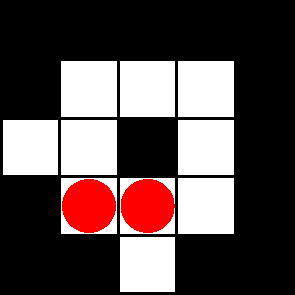
\includegraphics[width=0.8\textwidth]{one_way.pdf}
%    \caption{Reversible one-way gadget.}
%    \label{ldeScreenshotsMap}
%\end{figure}

\subsection{Set-Verify Gadgets}
For the Set-Verify gadget, the $S_i$ entrance is the only one which allows the robot to move any blocks. From the $S_i$ entrance they can traverse to $S_o$, and they can also pull the middle block down behind them. Doing so will allow a traversal from $V_i$ to $V_o$. To traverse back from $S_o$ to $S_i$, the robot must first traverse back from $V_o$ to $V_i$. Then, when the robot travels back from $S_o$ to $S_i$, they must push the middle block back, ensuring the $V_i$ to $V_o$ traversal is impossible. Further, access to any sequence of entrances will not allow the robot to alter the system to allow traversals between the $V_i$ and $S_i$ entrances. \\

There are four possible states of the Set-Verify: Broken, Unset, Set, and Verified. In the Broken state, the only possible transition is $S_o \rightarrow S_i$, changing the state to Unset. This state can only be reached from Unset, and allows strictly less future transtions than Set, which can also be reached from Unset, so we will disregard it. In the Unset state, the $S_i \rightarrow S_o$ transition is the only possibility, changing the state to Set. In the Set state, the $S_o \rightarrow S_i$ transition is possible, changing the state back to Unset, as well as the $V_i \rightarrow V_o$ transition, which changes the state to Verified. Finally, from the Verified state, the only transitions possible are $V_o \rightarrow V_i$, changing the state back to Set, and $V_i \rightarrow V_o$, leaving the state as Verify.

Since the Set-Verify gadget has no hallways with length greater than 3, any capabilities the robot may have of pushing or pulling more than one block at a time are irrelevant. Thus, the following proof will apply for all values of $j$ and $k$ in Push-$j$ Pull-$k$.

\begin{figure}[!ht]
  \centering
  \caption{Set-Verify Gadgets}
  \begin{subfigure}[b]{0.3\textwidth}
    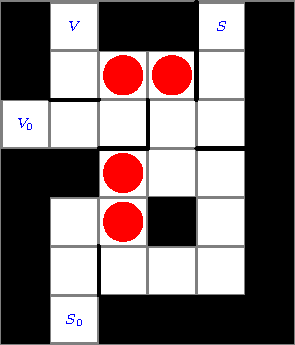
\includegraphics[width=\textwidth]{SetVerifyUnset}
    \caption{Set-Verify, unset state.}
    \label{ldeDiagrams}
  \end{subfigure}
  \begin{subfigure}[b]{0.3\textwidth}
    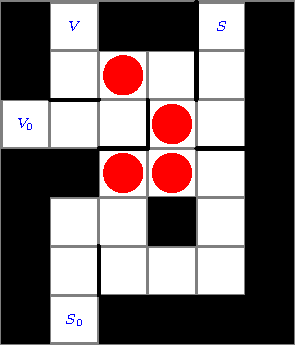
\includegraphics[width=\textwidth]{SetVerifySet}
    \caption{Set-Verify, set state.}
    \label{ldeDiagrams}
  \end{subfigure}
  \begin{subfigure}[b]{0.3\textwidth}
    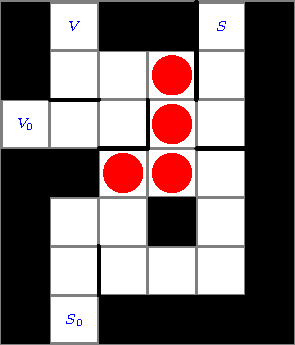
\includegraphics[width=\textwidth]{SetVerifyVerified}
    \caption{Set-Verify, verified state.}
    \label{ldeDiagrams}
  \end{subfigure}
\end{figure}

\subsection{Directed Destructive Crossover}
Initially this gadget allows either a traversal from $a$ to $a'$ or $b$ to $b'$. Once a traversal has occurred, that path may be traversed in reverse, but the other is impassable unless the original traversal is undone.

First, observe that transitions are initially only possible via the $a$ and $b$ entrances, since the transitions possible through a Set-Verify in state Set can be entered through $V_i$ and $S_o$, not $S_i$.

Assume without loss of generality that the gadget is entered at $a$. This changes the state of the left Set-Verify to Unset. At this point, the right $V_i$ transition is passable, as well as the left $S_i$ transition, and no others. Taking the $S_i$ transition reverts all changes to the original state. Taking the $V_i$ transition changes the right Set-Verify to Verified, and completes the crossover. At this point, the only possible transition is to undo the transition just made, from $a'$ back to $a$, restoring the original state. Thus, the only transition possibilities are as stated above.

\begin{figure}[!ht]
  \centering
  \caption{Two types of crossover gadgets}
  \begin{subfigure}[b]{0.45\textwidth}
    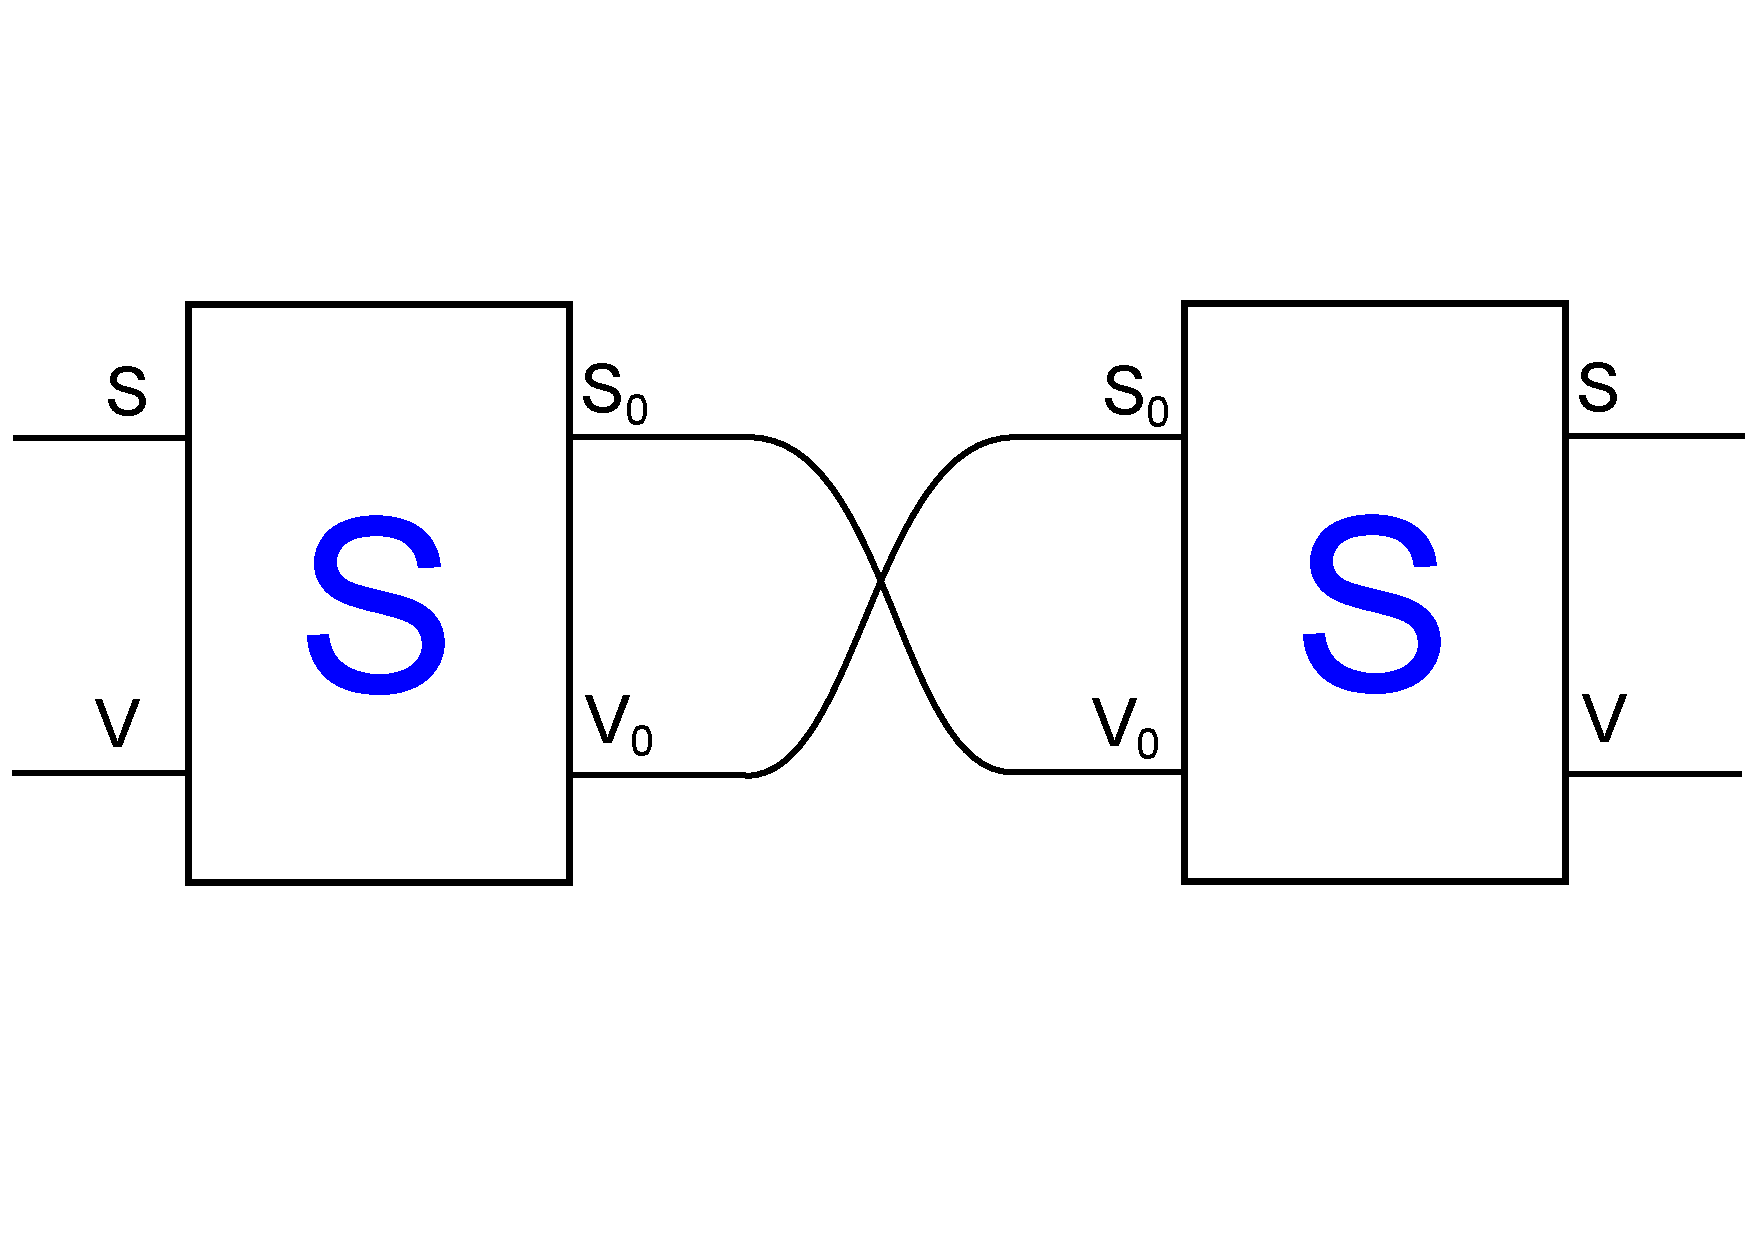
\includegraphics[width=\textwidth]{DestructiveCrossover}
    \caption{The one-way destructive crossover constructed from two connected Set-Verify gadgets initialized in the set position.}
    \label{DestructiveCrossover}
  \end{subfigure}
  \hfill
  \begin{subfigure}[b]{0.45\textwidth}
    \includegraphics[width=\textwidth]{InOrderCrossover}
    \caption{The in-order one-way crossover constructed from two connected Set-Verify gadgets initialized in the verified and unset positions.}
    \label{InOrderCrossover}
  \end{subfigure}
\end{figure}

\begin{figure}[!ht]
  \centering
  \caption{Two types of crossover gadgets}
  \begin{subfigure}[b]{0.9\textwidth}
    \includegraphics[width=\textwidth]{np_crossover}
    \caption{The one-use one-way crossover is constructed from a one-way destructive crossover and two in-order one-way crossovers}
    \label{OneUseCrossover}
  \end{subfigure}
\end{figure}

\subsection{In-order Directed Crossover}
This gadget allows a traversal from $a$ to $a'$, followed by a traversal from $b$ to $b'$.

Initially, no entrance is passable except for $a$, since $V_o$ is passable only in state Verifed, and $S_o$ is
passable only in state Set. Once the left $V_o \rightarrow V_i$ transition is made, the robot has 2 options.
It can either change the left Set-Verify's state to Set, or leave it as Verified. In either case, the $S_i$
entrance on that toggle is impassable, since a $S_i$ entrance may only be traversed in state Unset. The
only transition possible on the right crossover is $S_i \rightarrow S_o$, changing the state from Unset to Set.
This completes the first crossing.

Now, there are at most 2 transitions possible: from $a'$ back to $a$, undoing the whole process, or entering at $b$. Note that entering at $b$ is only possible if the left Set-Verify is in the Set state, so let us assume that state change occurred. In that case, the left $S_o \rightarrow S_i$ transition may be performed, changing the left Set-Verify's state to Unset. At that point, the only possible transitions are back to $b$, or through the right Set-Verify's
$V_i \rightarrow V_o$ transition, completing the second crossover.


\subsection{Directed Crossover}
This is the gadget needed for our proof. It allows a traversal from $a$ to $a'$ followed by a traversal from $b$ to $b'$, or a traversal from $b$ to $b'$.

It is constructed out of an In-order Directed Crossover gadget and a Destructive Directed Crossover, as shown in Figure \ref{OneUseCrossover}. The $a$ to $a'$ traversal is initially passable, and goes through both gadgets,
blocking the destructive crossover but leaving the in-order crossover open for the $b$ to $b'$ traversal. If the $a$ to $a'$ traversal does not occur, the $b$ to $b'$ traversal is possible via the destructive crossover.

\subsection{Crossover}
Four Directed Crossovers can be combined, as shown below, to create a crossover that can be traversed in any direction.

\subsection{3-SAT Construction}

\begin{figure}[!ht]
  \centering
  \begin{subfigure}[b]{0.9\textwidth}
    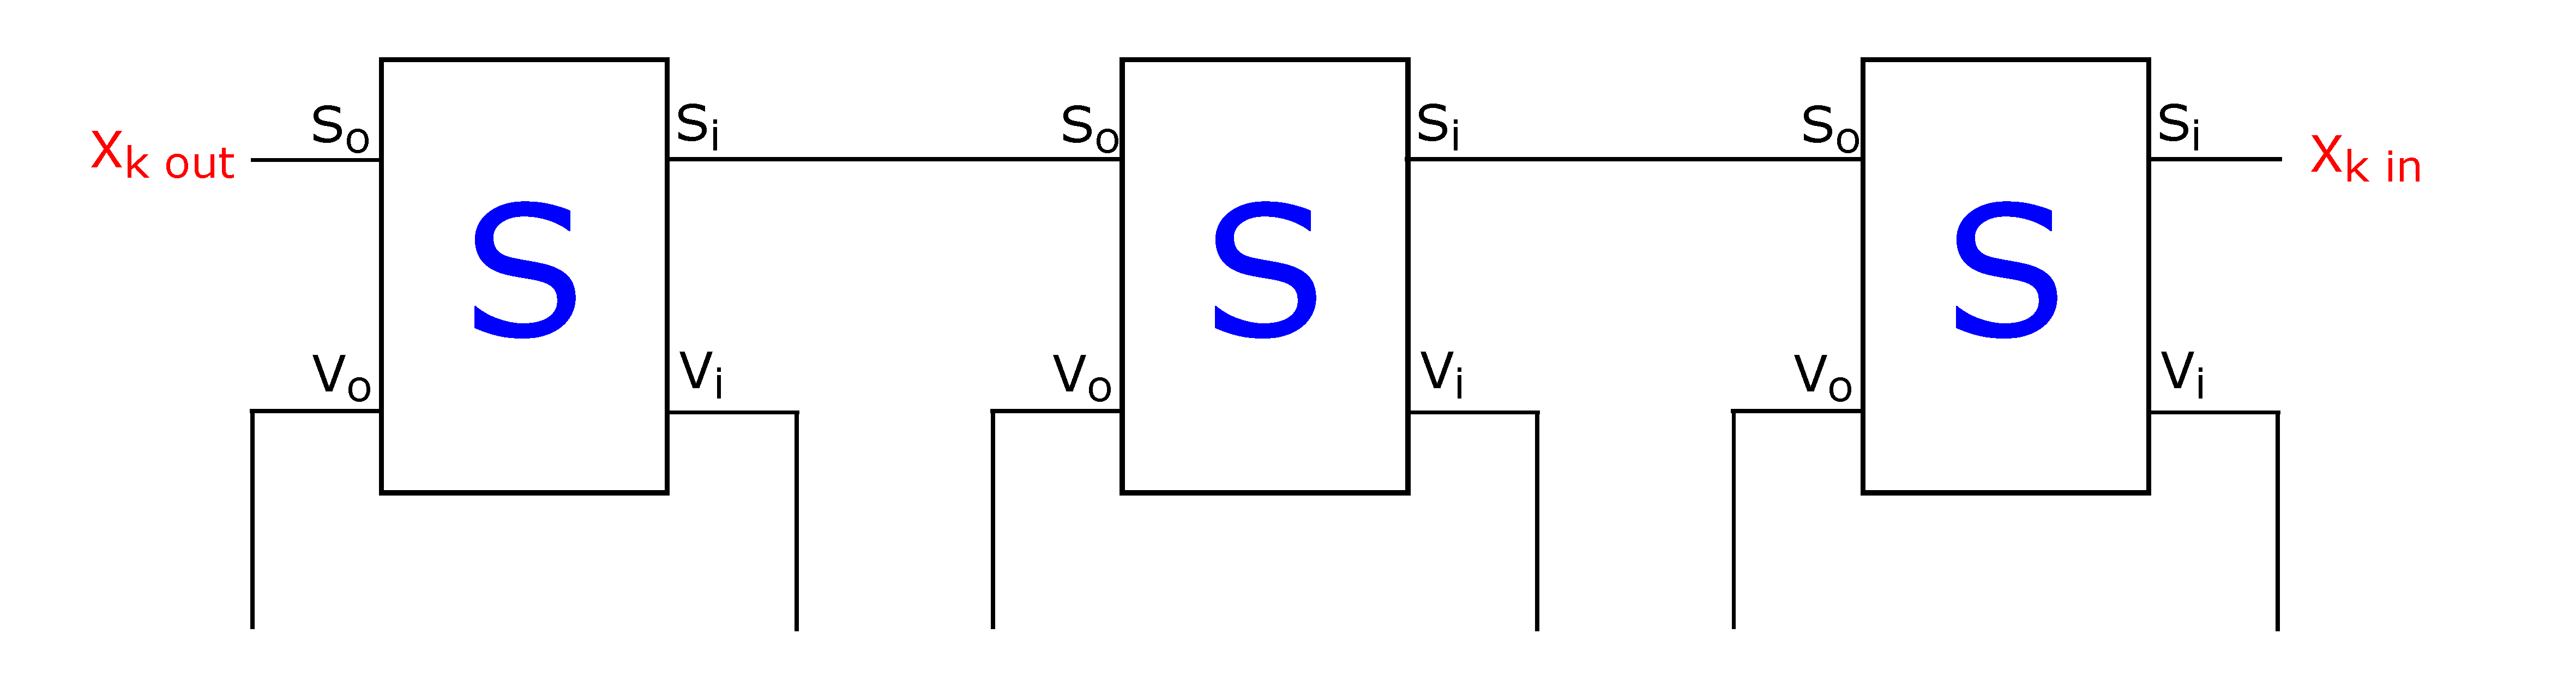
\includegraphics[width=\textwidth]{NPVariableGadget}
    \caption{variable}
    \label{NPVariableGadget}
  \end{subfigure}
\end{figure}

\begin{figure}[!ht]
  \centering
  \begin{subfigure}[b]{0.9\textwidth}
    \includegraphics[width=\textwidth]{NPClauseGadget}
    \caption{Clause}
    \label{NPClauseGadget}
  \end{subfigure}
\end{figure}

We plan to reduce from 3-SAT and will be making use of the Set-Verify gadget to produce our literals. One significant difficulty with this model is the complete reversibility of all actions. Thus we need to take care to ensure that going backward at any point does not allow the robot to cheat in solving our 3-SAT instance. The directional properties of the Set-Verify allow us to create sections where we know if the robot exits, it must have either reset everything to the initial configuration or put everything in another known state.

Our literals will be represented by Set-Verify gadgets. They are considered true when the $V_i$ to $V_o$ traversal is possible, and false otherwise. Thus we can set literals to true by allowing the robot to run through the $S_i$ to $S_o$ passage of the gadget. This implies a very simple clause gadget, consisting of splitting the path into three hallways each with the corresponding verify side of our literal. We can then pass through if any of the literals is set true and cannot be passed otherwise.

The variables will be encoded by a series of passages which split to allow either the true or negated literals to be set. Once variables split into two hallways, we have to show that when you enter or exit a side of a hallway, all the literals are set true at one end and false at the other. Also, we cannot go back through the other hallway, so if we go backward, everything gets reset. Thus we cannot exploit the reversibility to set anything extra true.

Therefore, in order to traverse all of the clause and reach the goal location, the robot must traverse a set of veriable hallways that encode an accepting assignment to the 3SAT problem, thus reducing 3SAT to this problem.

\section{PSpace}

\xxx{Introduction Needed}

\subsection{Toggles}
We define an $n$-toggle to be a gadget which has $n$ internal pathways and can be in one of two internal states, $A$ or $B$. Each pathway has a side labeled $A$ and another labeled $B$. When the toggle is in the $A$ state, the pathways can only be traversed from $A$ to $B$ and similarly in the $B$ state they can only be traversed from $B$ to $A$. Whenever a pathway is traversed the state of the Toggle flips.

%There is no no border on this figure, which looks weird.

\begin{figure}[!ht]
\centering
\begin{subfigure}[b]{0.45\textwidth}
  \centering
    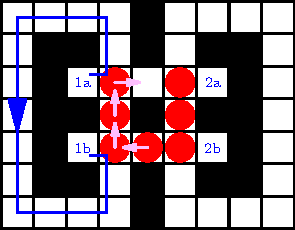
\includegraphics[width=0.8\textwidth]{2-toggleA}
    \caption{2-Toggle in state A}
    \label{2toggleA}
\end{subfigure}

\begin{subfigure}[b]{0.45\textwidth}
  \centering
    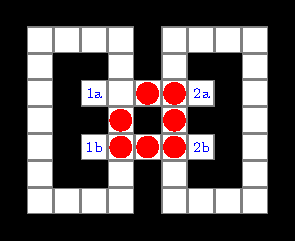
\includegraphics[width=0.8\textwidth]{broken2Toggle}
    \caption{2-Toggle in a broken state}
    \label{broken2toggle}
    \end{subfigure}
\end{figure}

\begin{figure}[!ht]
  \centering
    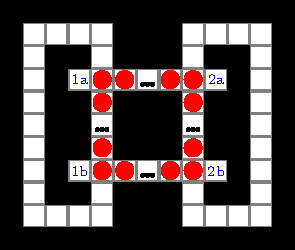
\includegraphics[width=0.8\textwidth]{2ToggleK}
    \caption{Construction of a 2-toggle when the robot can push or pull multiple blocks.}
    \label{2ToggleK}
\end{figure}

Figure \ref{2toggleA} acts as a 2-Toggle. Notice that there is a single block missing from the ring of eight blocks. When the missing block is on top, as diagrammed, it will represent state $A$, and when it is on the opposite side, we call it state $B$. Notice that in state $A$, it is impossible to enter through entries $1b$ or $2b$. When we enter in the $1a$ or $2a$ sides, we can follow the moves in the series of diagrams to exit the corresponding $1b$ or $2b$ side and leaving the gadget in the $B$ state. One can easily check that the gadget can only be left in either state $A$, $B$, or a broken state as seen in Figure \ref{brokenToggle}. Notice, in the broken state, every pathway except the one just exited is blocked. If we enter through that path, it is in exactly the same state as if it had been in an allowed state and entered through the corresponding pathway normally. For example, in the diagram one can only enter through $1b$ and after doing so it is the same as entering in path $1b$ on a 2-Toggle in state $B$. Thus the broken state is never useful for solving the puzzle and can be safely ignored.

\begin{figure}[!ht]
  \centering
  \begin{subfigure}[b]{0.45\textwidth}
    %\includegraphics[width=\textwidth]{4Toggle3D}
    \caption{Diagram of a 4-toggle}
    \label{4Toggle3D}
  \end{subfigure}
  \hfill
  \begin{subfigure}[b]{0.45\textwidth}
    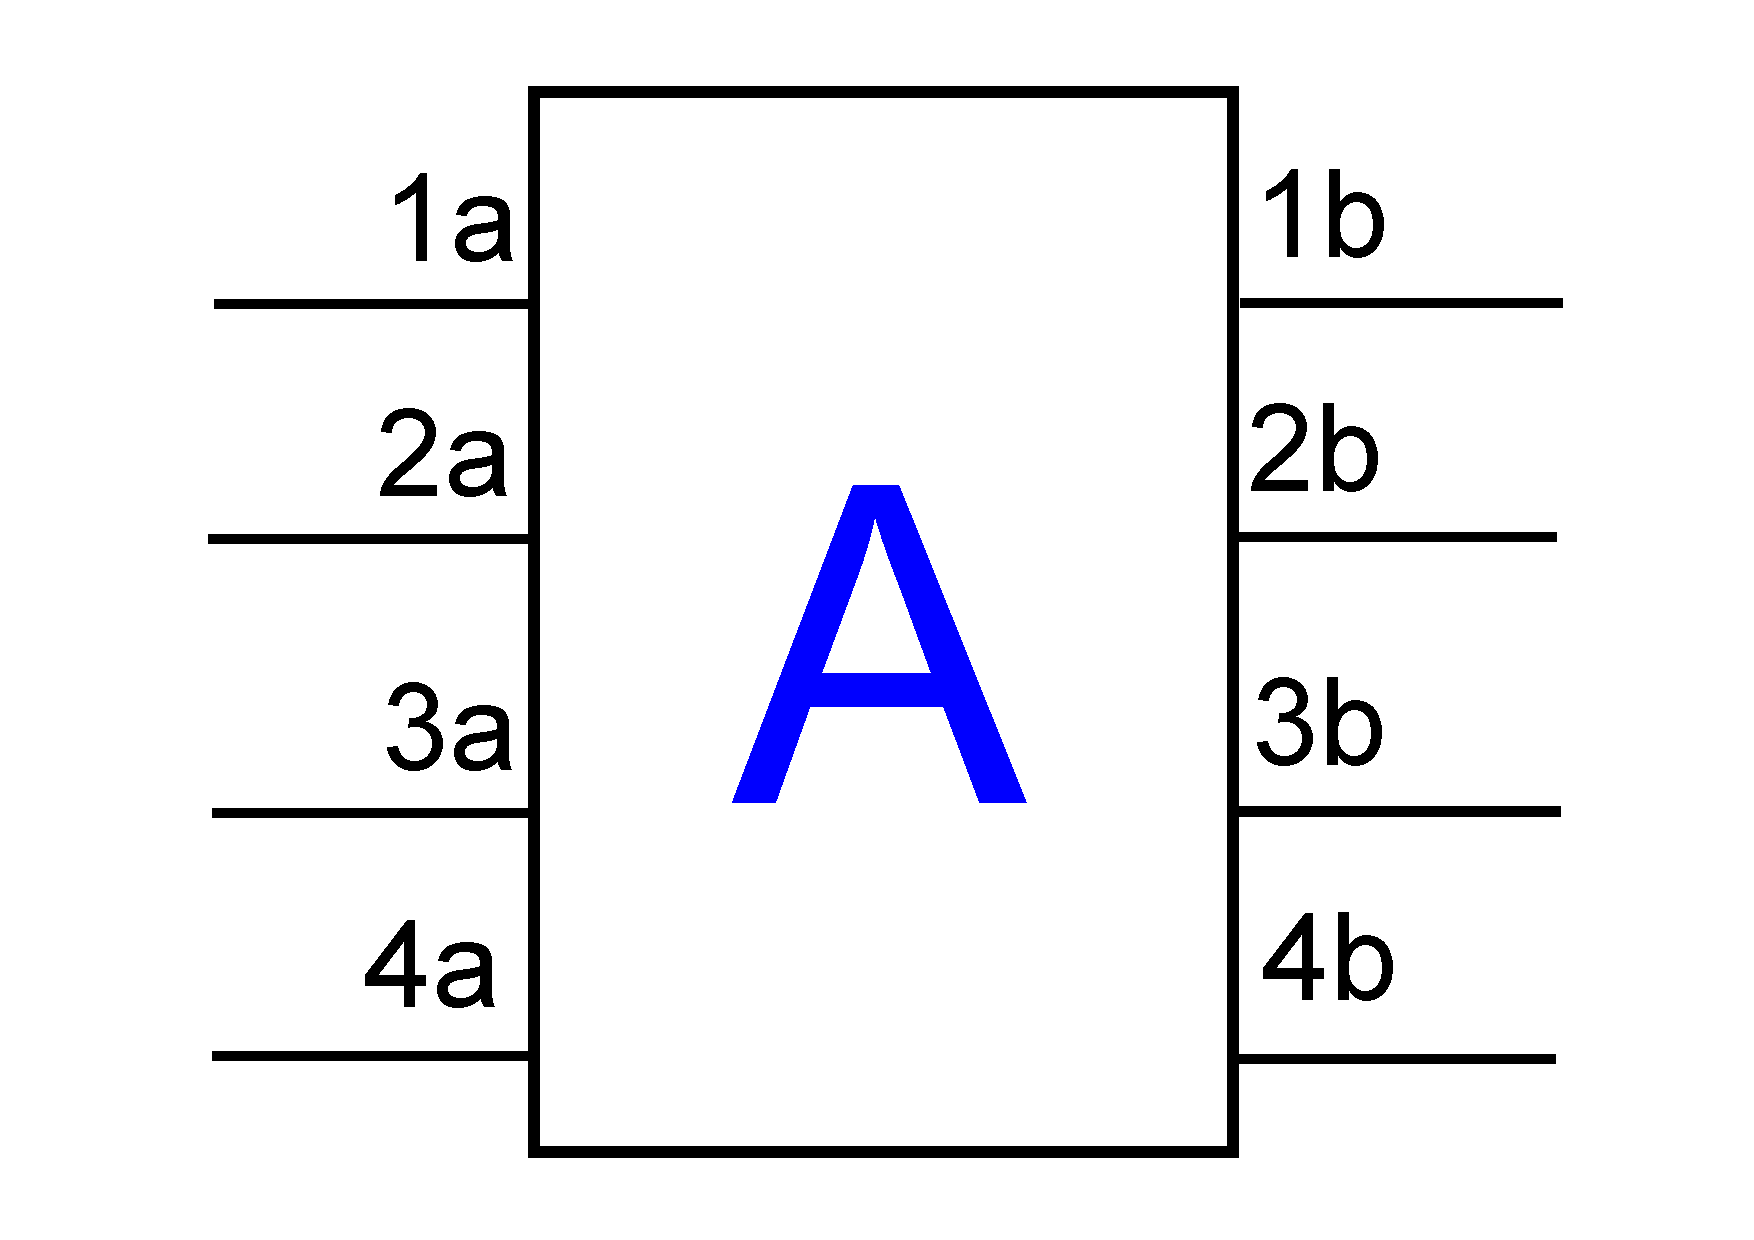
\includegraphics[width=\textwidth]{4Toggle}
    \caption{Representation of a 4-toggle in the $A$ state.}
    \label{4ToggleAbstract}
  \end{subfigure}
\end{figure}

To construct a 4-Toggle we essentially take two copies of the two toggle, rotate them perpendicular to each other in 3D, and let them overlap on the central axis. See Figure \ref{4Toggle}. We still interpret the lack of blocks in the same positions as the 2-Toggle as states $A$ or $B$. Now we have four different paths which function the same as the ones described above. Similar arguments show the broken states of the 4-Toggle also don't matter.

\section{Locks}

\xxx{lock figure}

A lock is a gadget consisting of a 2-toggle and a separate pathway. Traversing the separate pathway can only be done in a single direction, based on whether the 2-toggle is in state A or B, and the traversal does not change the internal state of the 2-toggle. The 2-toggle functions exactly
as described above. This gadget can be implemented using a 4-toggle, by
connecting the $3B$ and $4B$ entrances of the 4-toggle with an additional corridor, as shown in \ref{lock}.
Traversing the resultant full pathway, from $3A$ to $3B$ to $4B$ to $4A$, is possible only if the initial
state of the 4-toggle is $A$, and will leave the 4-toggle in state $A$. In addition, a partial traversal,
such as from $3A$ to $3B$ and back to $3A$, does not change the internal state. The two unaffected
pathways of the toggle, $1$ and $2$, continue to function as a 2-toggle.

A synchronized lock block is a gadget consisting of a 2-toggle and any number of separate pathways. As in the
lock, the 2-toggle functions as described above. Each pathway may be set up to be passable in either direction
if the toggle is in state $A$ and impassable in either direction if the toggle is in state $B$ (type A), or
passable in either direction if the toggle is in state $B$ and impassable in either direction if the
toggle is in state $A$ (type B). This is
implemented using one lock per non-toggling pathway needed. As shown in \ref{lockChain}, there are 2
pathways of the entire synchronized lock block system: the 1 pathway, and the 2 pathway. A lock whose pathway will create
a type A synchronized lock pathway is placed so that its pathways are in the same direction as the synchronized lock block's
pathways, $A$ entrance in the $A$ direction and $B$ entrance in the $B$ direction. Its state matches the 
synchronized lock block's
state.
A type $B$ lock is placed in the opposite direction, with its $B$ entrance in the synchronized lock block's $A$ direction and
A entrance in the B direction. Its state is also opposite the synchronized lock block's state.

When the synchronized lock block is traversed, all of the internal locks' states flip, rendering the synchronized lock block passable in
the opposite direction, and switching the passability and impassibility of all of the external pathways.

\subsection{Binary Counter}
\xxx{binary counter figure}
We now define a binary counter. The binary counter has a fixed number of internal bits.
Whenever the binary counter is traversed in the forwards direction, the binary number
formed by the internal bits increases by one and the robot leaves via one of the exits.
If the binary counter is traversed in the reverse direction, the internal value is reduced by
one. If the binary counter is partial traversed, but then the robot leaves via its initial entrance,
the internal value does not change.

The binary counter is implemented as a series of 2-toggles, as shown in \ref{binaryCounter}.
The entrance pathway is connected to the 2-toggle's $1A$ and $2B$ entrances. The $1B$ exit from the 2-toggle
will exit from the entire binary counter. The $2A$ exit will continue on to the next 2-toggle,
attaching to that toggle's $1A$ and $2B$ entrances. This will continue for every toggle down the line, except
that the last toggle's $2A$ exit signals an overflow, and exits from the counter.

To see that this produces the desired effect, identify a toggle in state $A$ as a $0$ bit, and a toggle in state
$B$ as a $1$ bit. Let the entrance toggle's bit be the least significant bit, and the final toggle be the
most significant. When the robot enters the binary counter in the forwards direction, it will flip
the state of every toggle it passes through. When it enters a toggle that is initially in state $B$, and thus whose
bit is $1$, it will flip the state/bit and proceed to the next toggle, via the $2B - 2A$ pathway. When it
encounters a toggle that is initial in state $A$ / bit $0$, it will flip the state/bit and exit, via the $1A - 1B$
pathway. Thus, the overall effect on the bits of the binary counter is to change a sequence of bits ending at the
least significant bit from $01..11$ to $10..00$. This has the effect of increasing the value of the binary counter
by one.

If the robot approaches this apparatus from the exit side, there are three possibilities. If the robot attempts
to enter via a $1B$ pathway whose toggle is in state $A$ / $0$, the toggle is impassable and the robot makes
no progress. If the robot enters via a $1B$ pathway whose toggle is in state $B$ / $1$, after traversal the
robot will have 2 options: To return in the direction it came, or to continue through the next toggle's
$2A -2B$ pathway. The latter is only possible if the next toggle
(the one just less significant than the entrance) is
in state $A$ / $0$. Upon traversing that toggle, the robot will again be able to return from where it came, or
progress in the same fashion if the next toggle is in state $A$ / $0$. This will continue until the robot
either turns back, or exits out the main entrance.

Thus, if and only if the robot enters via the least significant toggle which is set to 1, the robot will be
able to leave out the main entrance. If the robot enters any other way, it will be forced to return via the
path it entered by, and undo all changes it has made.

The transformation on the bits caused by the only possible successful reverse traversal is to change $10 .. 00$
to $01 .. 11$, resulting in a decrement operation, as desired.

\subsection{Existential}
We now define an existential gadget. An existential gadget is like a synchronized lock block, except that instead of a
2-toggle, it has a single pathway which is always passable in both directions, and upon traversing the pathway
the robot may or may not change the internal state of the synchronized lock block, as it chooses.

\xxx{existential figure}

As shown in \ref{Existential}, an existential gadget consists of a synchronized lock block, and a pathway with access to all
four pathways of the 2-toggle component of the synchronized lock block. Upon traversing the main pathway, the robot may
choose to traverse the 2-toggle any number of times, leaving it in either state, as desired.

\subsection{Quantifier Chain}
\xxx{individual quantifier figure, and figure for them all hooked up.}

We now define a quantifier chain, as shown in \ref{Quantifier}. A quantifier chain implements a series of
alternating existential and universal variables, as well as external literal pathways, which may traversed
if and only if their corresponding variables are set to a pre-specified value.

Traversing the quantifier chain
repeatedly in the primary direction will cycle the universal variables through all $2^n$ possible settings.
Upon each traversal, an initial sequence of the universal variables will have their values flipped.
At that time, the robot will have the option to set a corresponding length sequence of existential variables arbitrarily, consisting
of the existentials nested within the universal variables whose values were flipped.

Traversing  the quantifier chain in the reverse direction is only the possible if the robot enters
via the lowest order universal toggle whose setting is $1$. The traversal will go back one setting in the
sequence of possible settings of the universal variables, and allow the robot to set all existential variables
corresponding to altered universal variables arbitrarily. No other existential variables can be changed.

There is also a special exit, the overflow exit, which can only be
reached after all of the universal variable settings have been traversed. 

A quantifier chain is implemented much like a binary counter, with some additions. Every universal variable will be represented by a synchronized lock block, where each individual lock will serve as a literal. The 2-toggle which are governing the progression through the synchronized lock blocks are hooked up in the same manner as the 2-toggles in a binary counter gadget. This forces the synchronized lock blocks to be set to the corresponding values in the simulated binary counter.

The next addition are the existential variables, which consist of existential gadgets placed just after the $2A$
exits of each universal variable,
and just before the $1A$ and $2B$ entrances of the the next universal variable, as shown
in \ref{Quantifier2}.

One potential flaw in the apparatus as described so far is that a robot could enter via an exit corresponding
to a highly significant universal variable set to $1$, alter its paired existential variable,
and then leave via the original entrance.
This must not happen for the existential counter to work properly, so a series of lock-chain pathways are added
to each of the exits from the quantifier. Recall from the description of the binary counter that the only
possible reverse traversal of the counter should be via entering at the lowest significance variable set to $1$.
To prevent
entry at higher-significance variables set to $1$, we will add a series of locks to
that exit which are only passable if
all lower-significance universal variables are set to $0$, as shown in \ref{QuantifierLockChains}.

This prevents the undesired high-significance existential alteration problem mentioned above, because
it is now impossible to enter the gadget via the higher-significance universal variables which are set to $1$,
because that entryway will have at least 1 closed lock on it, and so be impassable. However, this addition does
not affect the desired forward or backward transition, because the entrance/exit in question will have
all of its synchronized lock block external pathways in the passable state.

\subsection{Formula}
We now define a clause gadget, as shown in \ref{Clause}. A clause gadget is a single pathway which is passable
if and only if at least one of 3 literals are passable. Recall from above that a literal is a pathway which is
passable if and only if a specified variable has a specified setting.

The formula gadget consists of a series of clauses, as shown in \ref{Formula}. The formula is thus only passable
if every clause is passable, and thus if the corresponding $3CNF$ formula is true.

\subsection{Beginning and End Conditions}
The overall progression of the robot through the puzzle will start with the quantifier chain,
incrementing the universal variables and setting the appropriate existential variables arbitrarily; then to
traverse the formula gadget to verify that the formula is true under that setting; and repeating.

At the beginning of this procedure, the robot must be allowed to set all of the existential variables arbitrarily.
To ensure this, we will set up the quantifier gadget in the state $01 .. 11$, with all variables set to $1$
except the highest order one.  The highest order variable will be special, and will not be used in the $3CNF$
formula. The initial position of the robot will be at the entrance to the quantifier gadget. This will allow
the robot to flip every universal in the quantifier gadget, from $01 .. 11$ to $10 .. 00$, and accordingly
set every existential variable arbitrarily. To force the robot to go forward through the quantifier gadget,
instead of going backwards through the clause chain, we will add a literal onto the end of the formula gadget
which is passable if and only if the highest order variable is set to $1$.

After this set up, the robot will progress through through the loop consisting of the quantifier gadget and the
formula gadget, demonstrating the appropriate existential settings for each assignment of the universal
quantifiers.

After progressing through every possible state of the universal quantifiers, the universals will be in the
state $11 .. 11$. At this point, the robot may progress through the quantifier gadget and exit via its special
pathway,
the carry pathway of the highest order bit. This special pathway will lead to the goal location of the puzzle.
Thus, only by traversing the quantifier - formula loop repeatedly, and demonstrating the solution to the TQBF
problem,
will the robot be able to reach the goal. The robot may reach the goal if and only if the corresponding quantified
boolean formula is true.
\section{Conclusion}

\section{Open Questions}

\subsection{Block Pushing}
\begin{itemize}
\item Close NP, PSpace gap.
\item No thin walls
\item All movable blocks
\item Push-Push Pull (seen in Catherin-not quite since you can get on them, also Zelda?)
%%\item 1x1 Rush Hour
\end{itemize}

\section{Acknowledgments}


%Melissa and Gi?
%Video game company?

%%JIP Recriational Discrete Math. July 31.

% bibliography
\bibliographystyle{plain}
\bibliography{PortalBib}{}
\end{document}

